%!TEX root = ../main.tex

\section{Ferromagnets: Pd/Co/Pd sample}
\label{sec:ferromagnet}

The first sample consists of two thin layers of Palladium (paramagnetic) and one
layer of Cobalt (ferromagnetic) of variable thickness (\SI{0.3}{\nano\meter} - 
\SI{2}{\nano\meter}) labelled in the following as $d$. The crystal lattice of the 
trilayer system in total acts as a ferromagnet. The different magnetic properties of 
the sublattice however can cause strong changes in both magnitude and direction of 
magnetization in special cases. These effects will in part be analysed in this 
section.

Before the measurement data is evaluated the applied model is presented. The 
Kerr-angle that is measured as a function of external magnetic field is proportional
to the magnetic induction. We are therefore effectively measuring a magnetic 
hysteresis modulo some numerical constants. Expanding on the work in \cite{article}
we can therefore impose a model to analytically describe the hysteresis curve traced 
out by the Kerr-angle $\Upphi$ in varying magnetic fields. This model is presented in
\autoref{eq:hysteresis-model}.

\begin{equation}
\label{eq:hysteresis-model}
\Upphi(H) = \Upphi_s \tanh\left( A ( H \pm H_c ) \right) + \mu H.
\end{equation}

Here introduced are  several parameters that influence the shape of the hysteresis 
curve. 

\begin{itemize}
\item $\Upphi_s$ is the Kerr-angle at the saturation point. 
\item $A$\footnote{for lack of more fitting nomenclature in the literature} 
determines the magnetic hardness of the sample.
\item $\pm H_c$ is the coercive field strength, on the up/downsweep of $H$.
\item $\mu$ is the magnetic permeability of air.
\end{itemize}

The last term ($\,+\mu H\,$) in \autoref{eq:hysteresis-model} stems from the 
definition of magnetic induction ($\vec{B}=\mu(\vec{M}+\vec{H})\;$). In theory, it 
should be possible to extract information about the magnetic permeability from the
best fit value of $\mu$. In practice, effects caused for example by the layering of 
different magnetic materials make a prediction rather difficult. For the purpose of 
the following analysis, the exact value of $\mu$ is not important anyways.

Once the measurements of the Kerr-angle in relation to external magnetic field are
taken, the set of Kerr-angles is offset by its mean value. This eliminates systematic
errors in the data and helps to compare measurement values across the different 
measurement sets varying in Co-layer thickness $d$. This is the only correction 
applied to the dataset and is sufficient to make qualitative statements about the 
magnetic properties of the sample. The results of the analysis are presented in 
\autoref{fig:ferromagnet-measurement} and \autoref{tab:fitvals-ferro}.

At first glance, the results seem intuitive. For layer thicknesses of \SI{0.4}{\nano
\meter} to \SI{0.9}{\nano\meter} the magnetic properties such as coercive field 
strength or hardness of the material agree within an order of magnitude. Regarding 
the imperfections in both measurement apparatus and applied model, this implies 
the magnetic properties do not change. Only the Kerr-angle at saturation, $\Upphi_s$,
seems to display an upwards trend with increasing $d$. This is expected, since a
thicker layer allows for more domains to become magnetised, causing a higher net
magnetisation (and by extension Kerr-angle) at a given external magnetic field $H$.

The magnetic behaviour for thicker Co-layers drastically changes. As explained in the
lab manual, this is most likely caused by anisotropic effects near the boundaries of 
the different magnetic layers. For certain values of $d$, the magnetisation seems to 
point into the transversal direction of of the measurement plane (compare 
\autoref{fig:kerr1}). Under such circumstances, the magneto-optic Kerr effect 
disappears and a hysteresis is no longer visible. This culminates in unphysical fit
parameters for a Co-layer thickness of \SI{2.0}{\nano\meter}, where the fitting 
algorithm attempts to fit a hysteresis to a dataset that does not display any such 
behaviour and is purely dominated by the last term in \autoref{eq:hysteresis-model}.
For smaller layer thicknesses (\SI{1.4}{\nano\meter} and \SI{1.7}{\nano\meter}) this 
effect can already be observed in parts.

The effective anisotropy constant $K_\text{eff}$ helps quantifying the strength of
these boundary layer effects. The values of $K_\text{eff}$ for different Co-layer 
thicknesses are give in \autoref{tab:K-eff-ferromagnet}.

\begin{figure}
	\centering
	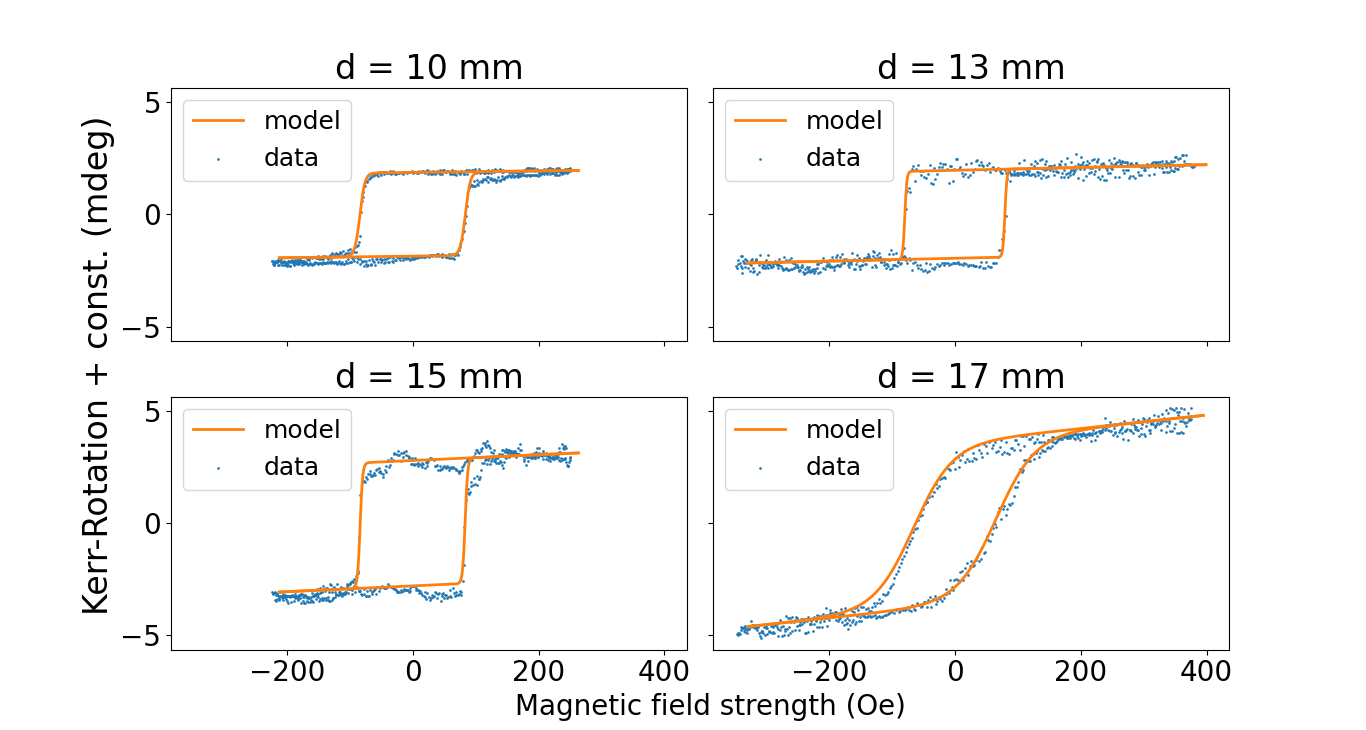
\includegraphics[width=1.0\textwidth]{./fig/ferromagnet_measurement.png}
	\caption{The hysteresis of a Pd/Co/Pd layer system for different Co-layer
	thicknesses.}
	\label{fig:ferromagnet-measurement}
\end{figure}

\begingroup
\renewcommand{\arraystretch}{1.1}
\begin{table}
	\begin{center}
	\caption{Hysteresis best fit values for different Co-layer thicknesses. Statistical errors estimated by the fitting algorithm are neglected due to their relative size being about $10^{-5}$. This does not accurately represent the true uncertainty of the dataset.}
	\begin{tabular*}{\textwidth}{@{\extracolsep{\fill}} c|cccc}
  \toprule
	\hline
  $d$ & $\Upphi_s$ & $A$ & $H_c$ & $\mu$ \\
	\hline
	\SI{0.4}{\nano\meter} & \SI{1.84}{\milli\degree} & \SI{121.3604}{\per\milli\oersted} & \SI{83.59}{\oersted} & \SI{0.84}{\micro\degree\per\oersted} \\
	\SI{0.5}{\nano\meter} & \SI{2.10}{\milli\degree} & \SI{260.5127}{\per\milli\oersted} & \SI{78.79}{\oersted} & \SI{0.18}{\micro\degree\per\oersted} \\
	\SI{0.7}{\nano\meter} & \SI{2.91}{\milli\degree} & \SI{152.2159}{\per\milli\oersted} & \SI{84.84}{\oersted} & \SI{0.77}{\micro\degree\per\oersted} \\
	\SI{0.9}{\nano\meter} & \SI{3.24}{\milli\degree} & \SI{19.1988}{\per\milli\oersted} & \SI{66.67}{\oersted} & \SI{4.44}{\micro\degree\per\oersted} \\
	\SI{1.4}{\nano\meter} & \SI{2.40}{\milli\degree} & \SI{10.9649}{\per\milli\oersted} & \SI{55.91}{\oersted} & \SI{4.54}{\micro\degree\per\oersted} \\
	\SI{2.0}{\nano\meter} & \SI{0.10}{\milli\degree} & \SI{1362.8763}{\per\milli\oersted} & \SI{-28.30}{\oersted} & \SI{2.79}{\micro\degree\per\oersted} \\
	\hline
	\bottomrule
	\end{tabular*}
	\label{tab:fitvals-ferro}
	\end{center}
\end{table}
\endgroup


\begingroup
\renewcommand{\arraystretch}{1.4}
\begin{table}
	\begin{center}
	\caption{Effective anisotropy constant in relation to Co-layer thickness}
	\begin{tabular*}{0.9\textwidth}{@{\extracolsep{\fill}} c|cccc}
  \toprule
	\hline
  $d$ & $\Upphi_s$ & $H_s$ & $H_c$ & $K_\text{eff} = -\frac{1}{2}\Upphi_s(H_s-H_c)$ \\
	\hline
	\SI{0.4}{\nano\meter} & \SI{1.84}{\milli\degree} & \SI{99.07}{\oersted} & \SI{83.59}{\oersted} & \SI{-14.25}{\milli\degree\per\oersted} \\
	\SI{0.5}{\nano\meter} & \SI{2.10}{\milli\degree} & \SI{89.68}{\oersted} & \SI{78.79}{\oersted} & \SI{-11.42}{\milli\degree\per\oersted} \\
	\SI{0.7}{\nano\meter} & \SI{2.91}{\milli\degree} & \SI{99.05}{\oersted} & \SI{84.84}{\oersted} & \SI{-20.67}{\milli\degree\per\oersted} \\
	\SI{0.9}{\nano\meter} & \SI{3.24}{\milli\degree} & \SI{127.52}{\oersted} & \SI{66.67}{\oersted} & \SI{-98.63}{\milli\degree\per\oersted} \\
	\SI{1.4}{\nano\meter} & \SI{2.40}{\milli\degree} & \SI{140.86}{\oersted} & \SI{55.91}{\oersted} & \SI{-101.89}{\milli\degree\per\oersted} \\
	\SI{2.0}{\nano\meter} & \SI{0.10}{\milli\degree} & \SI{-0.58}{\oersted} & \SI{-28.30}{\oersted} & \SI{-1.33}{\milli\degree\per\oersted} \\
  \bottomrule
	\end{tabular*}
	\label{tab:K-eff-ferromagnet}
	\end{center}
\end{table}
\endgroup

